\documentclass[11pt, twocolumn]{article}
\usepackage[utf8]{inputenc}
\usepackage[a4paper, margin=2cm]{geometry}
\usepackage[portuguese]{babel}
\usepackage{multicol}
\usepackage{graphicx}
\usepackage{tabularx}
\usepackage{abstract}
\usepackage{hyperref}
\usepackage[backend=biber, style=authoryear, sorting=nyt]{biblatex}
\addbibresource{refs.bib}

\begin{document}
\title{Relátio referente a construção do processador SAP1 em Python}
\author{Bruno Gomes}
\date{\today}
\twocolumn[
\maketitle
\begin{onecolabstract}
  Foi construído um processador virtual em Python que segue a arquitetura SAP1. Primeiramente foi criado um pacote em Python capaz de simular circuitos digitais e em seguida foi implementado uma micro-arquitetura conhecida para o SAP1. O processador foi testado e foi usado para rodar programas escritos em linguagem de maquína.
\end{onecolabstract} ]

\section{Introdução}
\subsection{Arquitetura}
   A arquitetura SAP1 é uma arquitetura de 8 bits com um conjunto de instruções minimo, essa arquitetura é apresentada por Malvino. A figura \ref{fig-blocks} é um diagrama de blocos da arquitetura, nota-se dois registradores conectados ao somador, um registrador de saida, banco de memória 4x8 bits e os demais componentes esperados como MAR, PC, CU. Todos os blocos de comunicam através de uma bus central (bus W), para que isso seja possível as saídas dos blocos devem usar lógica de três estados. O conjunto de instruções da arquitetura é apresentado na tabela \ref{tab-inst}, essas instruções são: ADD, LDA, SUB, HLT e OUT (a instrução OUT é omitida na construção do processador virtual). Percebe-se que essa arquitetura não apresenta nenhuma instrução de jump, o que limita muito o tipo de computação que pode ser feito, porém para fins de aprendizado isso é irrelevante. Todas as instruções seguem o mesmo formato, a instrução tem comprimento de 8 bits e é dividida em opcode (4 bits mais siginifactivos) e endereço (4 bits menos significativos).

   \begin{figure}
     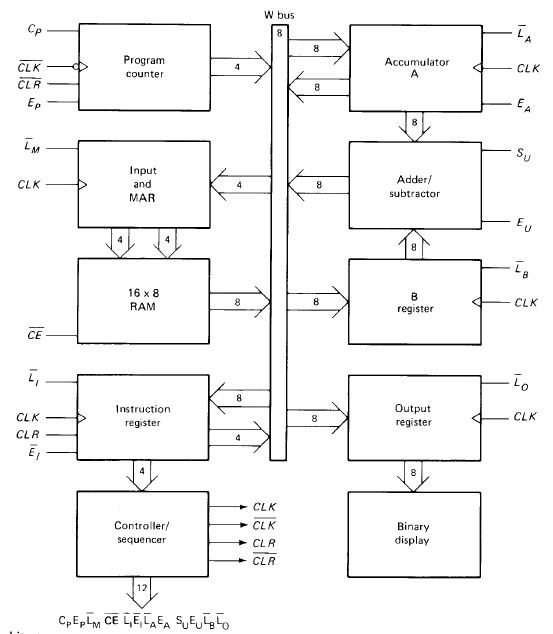
\includegraphics[width=0.5\textwidth]{blocks.jpg}
     \caption{Diagrama de blocos do processador SAP1. (Malvino)}
     \label{fig-blocks}
   \end{figure}
   
\subsection{Micro arquitetura}
A micro arquitetura construída foi baseada na implementação feita na literatura e tem como principal característica que cada instrução demora 6 ciclos do relógio para ser executada. A unidade de controle construída é diferente daquela apresentada por Malvino e recebe como entrada o ciclo da micro-instrução, gerado por um contador de 0 a 5 com um comparador que gera um sinal de reset, e o op-code da instrução; e como saída as 12 flags que controlam os blocos do processador. Intermamente a unidade de controle usa uma memória ROM como uma look-up table.

\begin{table}
  \caption{Instruções da arquitetura SAP1 e suas descrições.}
\begin{tabular*}{\linewidth}{lcp{5cm}}
  \hline
 Inst. & Op code & Descrição \\
 \hline
 LDA         &     0x0 & Carrega o acumulador com o valor contido no endereço dado. \\
 ADD         &     0x1 & Soma o valor presente no acumulador com o valor contido no endereço dado. \\
 SUB         &     0x2 & Subtrai o valor presente no acumulador com o valor contido no endereço dado.\\
 OUT         &     0xE & Escreve o valor contido no acumulador ao registro de saída (Out). \\ 
 \hline
\end{tabular*}
\label{tab-inst}
\end{table}


\subsection{PDD}
A implementação do processador foi feita usando o programa desenvolvido durante a fase inicial do projeto, a esse programa foi dado o nome PDD que atua como um simulador de circuitos digitais com sinais ideais.
PDD é escrito em Python puro e é distribuido como um pacote Python comum.
A descrição completa da arquitetura do simulador é complexa e foje do escopo desse artigo, porém as principais caractéristicas são instrutivas.
PDD foi construído com orientação a objetos em seu núcleo, novos circuitos são implementados pelo usuário de maneira direta utilizando o conceito de herança.
No momento PDD não possui um front-end que seja amigável a usuários inexperientes, porém é capaz de simular um processador como será demostrado.
PDD dispõe ao usuário os principais circuitos combinacionais, sequenciais e portas lógicas.

\section{Procedimento Experimental}
  
A fim de simplificar a construção do processador ele foi separado em duas partes que interagem entre si, bloco CU e SAU, fazendo uso da modularidade conceito esse muito usado no paradigma de circuitos digitais.
O bloco CU é a unidade de controle do processador e como entrada recebe o ciclo da micro instrução (ic) e o opcode da instrução sendo executada (iw); e como saída a palavra de controle que é aceita pela SAU para controlar os elementos do processador.
O bloco SAU contém todos os blocos presentes na figura \ref{fig-blocks} e adicionalmente um contador com circuito de reset responsável por gerar o sinal referente ao ciclo da micro instrução.
Como entrada SAU recebe um sinal de clock e reset (clk e r) e as diversas flags de controle; como saida recebe o ciclo da micro-instrução (ic), a bus de saída do registrador out e o opcode da intrução (iw).
A separação foi feita para facilitar no processo de desenvolvimento do processador pois tendo dois modulos bem definidos como a SAU e CU facilitam imensamente o processo de debugar, algo muito prezado durante o desenvolvimento do PDD, pois dessa forma cada bloco pode ser testado usando testes unitarios, conceito esse muito comum na programação.
A fígura \ref{fig-cu} apresenta um diagrama de blocos alternativo do processador usando os dois blocos definidos acima.

Como todo circuito em PDD, foi criado uma classe para o bloco CU com as entradas e saídas como descritas anteriormente, o endereço usado pela look-up table da CU é dado pela concatenção das buses ic e iw, a memoria tem como tamanho de palavra 12 bits, um bit para cada flag da SAU.
As micro instruções do processador e quais flags são ativas a cada ciclos está disponivel em \cite{malv}
A tabela \ref{tab-flags} lista as 12 flags e suas funções. 

\begin{table}
  \caption{Descrição das flags de controle do processador.}
\begin{tabular}{ll}
\hline
Flag & Descricao \\
\hline
cp & Incrementar PC no proximo clk \\
ep & Tristate de saida do PC \\
lm & Tristate de entrada do MAR \\
ce & Tristate saida da RAM \\
li & Tristate de entrada do IR \\
ei & Tristate de saida do IR \\
la & Tristate de entrada do acumulador \\
ea & Tristate de saida do acumulador \\
su & Flag de subtracao para o adder/subtractor \\
eu & Tristate de saida para o adder/subtractor \\
lb & Tristate de entrada para o registrador B \\
lo & Tristate de entrada para o registrador output \\
\hline
\end{tabular}
\label{tab-flags}
\end{table}

   \begin{figure}
     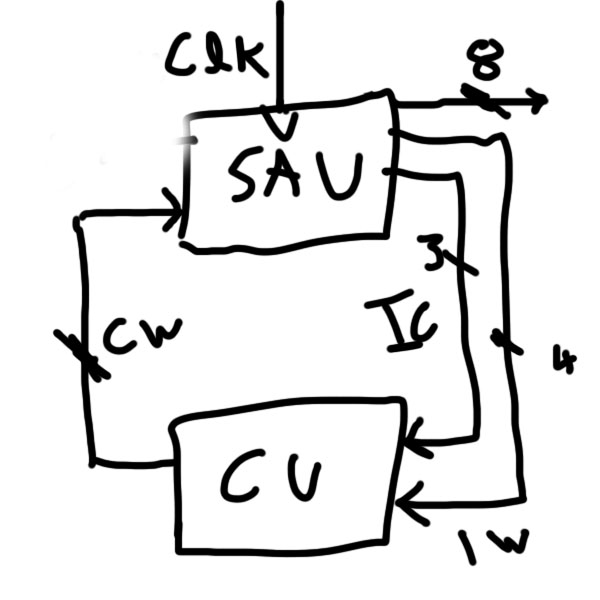
\includegraphics[width=0.5\textwidth]{cu.jpg}
     \caption{Diagrama de blocos ilustrando a conexão entre SAU e CU. Os sinais iw e ic são o op-code da instrução e o ciclo da micro-instrução, respectivamente, cw é a palavra de controle com as 12 flags referente aos blocos em SAU. Nota-se uma bus de saída em SAU de tamanho 8 referente ao registrador OUT.}
     \label{fig-cu}
   \end{figure}
 
O bloco SAU foi implementado da mesma maneira como pode ser visto na imagem \ref{fig-blocks} com a adição de um contador e um comparador que são responsáveis por marcar o ciclo das micro instruções, o comparador tem como uma das entradas o sinal $0x5$ e na outra o contador, sua saída é ligada à entrada de reset "r" do circuito contador.

Finalmente uma ultima classe referente ao processador foi criada.
A classe processador tem duas entradas: reset (r) e clock (clk) e uma unica saída, out. Internamente o processador é composto pelos blocos SAU e CU como foi apresentado na fig. \ref{fig-cu}. 

Para executar programas no processador foi escrito um arquivo de texto o conteúdo da memória interna, carregado através do método "fburn" da classe ROM, feito basta alternar o sinal na Bus clk entre 0 e 1, gerando assim um sinal de clock.

\section{Resultados}

Foram escritos 3 programas para o processador executar.
Os programas foram executados e foi inspecionado se o resultado escrito para no registrador "out" estava de acordo com o que era esperado.
O código fonte da implementação do processador e dos programas executados está disponível em \url{https://github.com/Lodek/pdd/tree/master/builds/sap1}.

\subsection{Programa 1}
O primeiro programa escrito simplemeste carrega um valor no registrador ACC com a instrução LDA e move esse valor para o registrador out com a instrução OUT.
As instruções do programa estão presentes na tabela \ref{tab-p1}. Nota-se que o programa é extremamente simples e foi usado para testar as instruções básicas.
O resultado esperado da execução do programa é que o valor no registrador out seja 3 e o resultado obtido está de acordo.

\begin{table}
  \caption{Palavras na memória para execuçao do programa 1}
\begin{tabular}{ll}
  \hline
  Endereço & mem. Conteúdo \\
  \hline
  0x0 & 0x0F \\
  0x1 & 0xE0 \\
  0x2 - 0xE & 0x0 \\
  0xF & 0x03 \\
  \hline
  \end{tabular}
\label{tab-p1}
\end{table}

\subsection{Programa 2}
O programa 2 testa a instruçao de addição.
O valor do inicial do acumulador (0) é somado ao valor presente do endereço 0xF (valor 3), em seguida o valor presente no acumulador (3) é escrito no registrador de saída.
O resultado obtido foi $3$, como esperado.

\begin{table}
  \caption{Palavras na memória para execuçao do programa 2.}
\begin{tabular}{ll}
  \hline
  Endereço mem. & Conteúdo \\
  \hline
  0x0 & 0x1F \\
  0x1 & 0xE0 \\
  0x2 - 0xE & 0x0 \\
  0xF & 0x03 \\
  \hline
  \end{tabular}
\label{tab-p2}
\end{table}

\subsection{Programa 3}
O terceiro e ultímo programa executado utiliza todas a instruções do processador e combina-as em um uníco programa.
Primeiramente o valor 3 é carregado no acumulador, em seguida é o valor 6 é somado ao valor no acumulador, subtrai-se 2 do acumulador e finalmente o resultado é escrito no registrador out.
O resultado obtido foi 7, demonstrando que o processador está executando todas as intruções corretamente.

\begin{table}
  \caption{Palavras na memória para execuçao do programa 3}
\begin{tabular}{ll}
  \hline
  Endereço mem. & Conteúdo \\
  \hline
  0x0 & 0x0F \\
  0x1 & 0x1E \\
  0x2 & 0x2D \\
  0x3 & 0xE0 \\
  0x4 - 0xC & 0x0 \\
  0xD & 0x02 \\
  0xE & 0x06 \\
  0xF & 0x03 \\
  \hline
  \end{tabular}
\end{table}
\label{tab-p3}


\section{Conlusão}

A ferramenta PDD possibilita a simulação de circuitos digitais e foi utilizado para replicar a arquitetura descrita na literatura.
A arquitetura escolhida é simples porém a base de qualquer arquitetura está presente nela, sendo assim é possivel utilizar a mesma ferramenta para simular uma arquitetura mais completa (mais instruções) e diferentes tamanhos de palavras.
PDD foi capaz de simular o processador, executar corretamente os programas escritos e como resultado obteve a resposta ao problema.

O objetivo da ferramente construida é respeitar os principios dos circuitos digitais, gerar uma abstração que seja familiar para estudantes com expêriencia em montar circuitos em protoboards e possibilitar a construção de circuitos digitais abstratos usando os principios da programação orientada a objetos.

Um grande defeito de PDD é velocidade, devido à estrutura dada ao aplicativo pode-se notar uma performance que se deixa a desejar,
para corrigir esses problema existem varias alternativas. Primeiramente poderia reduzir redundância devido aos eventos através de caches, evitando assim que circuitos sejam atualizados desnecessariamente.
Pode-se tambem utilizar algoritimos mais sofisticados e paralelismo para realizar as operações.
Finalmente seria possivel optar por uma implementação mais rápida dos blocos sequências e combinacionais presentes no pacote PDD; atualmente esses blocos foram construídos usando nada além das portas lógicas presentes no PDD, isso é ineficiente pois ao invez de ser usado os circuitos já presentes no processador do host PDD está emulando isso. 

\printbibliography

\end{document}
